\documentclass{beamer}
\useoutertheme{shadow}
\usepackage{tabularx}
\usetheme{Madrid}
\usepackage{tikz}
\usetikzlibrary{positioning, fit, arrows.meta, shapes}
\usepackage{caption}
\usepackage{subcaption}

\AtBeginSection{\frame{\sectionpage}}
\defbeamertemplate{section page}{custom}[1][]{%
  \begin{centering}
    {\usebeamerfont{section name}\usebeamercolor[fg]{section name}#1}
    \vskip1em\par
    \begin{beamercolorbox}[sep=12pt,center]{part title}
      \usebeamerfont{section title}\insertsection\par
    \end{beamercolorbox}
  \end{centering}
}
\setbeamertemplate{section page}[custom]

\newcommand{\R}{\mathbb{R}}
\newcommand{\N}{\mathbb{N}}
\newcommand{\empt}[2]{$#1^{\langle #2 \rangle}$}
\setbeamertemplate{section in toc}{\inserttocsectionnumber.~\inserttocsection}

\definecolor{mvablue}{rgb}{0.1098, 0.1373, 0.5137}
\definecolor{mvapurple}{rgb}{0.3373, 0.1529, 0.4510}
\definecolor{mvared}{rgb}{0.5725, 0.1882, 0.3922}

\colorlet{titleleft}{mvablue}
\colorlet{titlemiddle}{mvapurple}
\colorlet{titleright}{mvared}
\DeclareMathOperator{\leakyrelu}{LeakyReLU}

\pgfdeclarehorizontalshading[titleleft,titlemiddle,titleright]
      {beamer@frametitleshade}{\paperheight}{
    color(0pt)=(titleleft);
    color(0.5\paperwidth)=(titlemiddle);
    color(\paperwidth)=(titleright)
  }

\useinnertheme{tcolorbox}
\addtobeamertemplate{title}{
  \begingroup
  \tcbset{
    enhanced,
    interior style={left color=mvablue,right color=mvared}
  }
}{\endgroup}

\addtobeamertemplate{section page}{
  \begingroup
  \tcbset{
    enhanced,
    interior style={left color=mvablue,right color=mvared}
  }
}{\endgroup}

\title{CFM Data Challenge}
\subtitle{\textit{Stock Classification from High Frequency Market Data}}

\author{Sofiane Ezzehi \and Bastien Le Chenadec}
\institute[MVA]{École Normale Supérieure Paris-Saclay, Master MVA}
\date{March 20th, 2024}

\logo{
\includegraphics[width=0.6cm]{figures/MVA-logo.png}}

\setbeamercolor{author in head/foot}{parent=palette primary,bg=}
\setbeamercolor{title in head/foot}{parent=palette secondary,bg=}

\makeatletter
\setbeamertemplate{footline}
{
    \leavevmode%
    \setbox\beamer@tempbox=\hbox{%
        \begin{beamercolorbox}[wd=.5\paperwidth,ht=2.25ex,dp=1ex,center]{author in head/foot}%
            \usebeamerfont{author in head/foot}\insertshortauthor\expandafter\beamer@ifempty\expandafter{\beamer@shortinstitute}{}{~~(\insertshortinstitute)}
        \end{beamercolorbox}%
        \begin{beamercolorbox}[wd=.5\paperwidth,ht=2.25ex,dp=1ex,center]{title in head/foot}%
            \usebeamerfont{title in head/foot}\insertshorttitle
        \end{beamercolorbox}%
        }%
        \beamer@tempdim=\ht\beamer@tempbox%
        \advance\beamer@tempdim by 4pt%
        \begin{pgfpicture}{0pt}{0pt}{\paperwidth}{10pt}
            \pgfpathrectangle{\pgfpointorigin}{\pgfpoint{\paperwidth}{\beamer@tempdim}}
            \pgfusepath{clip}
            \pgftext[left,base]{\pgfuseshading{beamer@frametitleshade}}
        \end{pgfpicture}
        \vskip-\beamer@tempdim%
        \box\beamer@tempbox%
}%
\makeatother

\newcommand{\myitem}{\item[$\rightarrow$]}
\newcommand{\mycoolitem}{\item[\checkmark]}

\begin{document}
\frame[plain]{\titlepage}

\begin{frame}
    \frametitle{Table of contents}
    \small\tableofcontents[subsectionstyle=hide]
\end{frame}

\section{Introduction}
\begin{frame}{Introduction}
    \begin{itemize}
        \item \textbf{Objective:} Classify stocks based on snapshots of their respective order books.
        \item \textbf{Data:} Each sample is a 100-event sequence of the posted \textbf{passive} and \textbf{aggressive} orders in the order book.
        \item A lot of usual features are \textbf{missing}, and others are \textbf{hidden}. \textit{Example : The Price, best bid and best ask are centered around the first event.}
    \end{itemize}
    % \begin{itemize}
    %     \item \textbf{Stocks:} 24
    %     \item \textbf{Events:} 100
    %     \item \textbf{Train samples:} 160,800 samples
    %     \item \textbf{Test samples:} 80,600 samples
    % \end{itemize}

    % put the data in a table
    \begin{table}[H]
        \begin{center}
            \begin{tabular}{|c|c|c|c|c|}
                \hline
                \textbf{}       & \textbf{Stocks} & \textbf{Events} & \textbf{Train samples} & \textbf{Test samples} \\
                \hline
                \textbf{Number} & 24              & 100             & 160,800                & 80,600                \\
                \hline
            \end{tabular}
        \end{center}
    \end{table}

\end{frame}

\begin{frame}{Data Overview}

    \begin{table}[H]
        \tiny
        \begin{center}
            \resizebox{\columnwidth}{!}{
                \begin{tabular}{|c|c|p{5cm}|}
                    \hline
                    \textbf{Feature} & \textbf{Type} & \textbf{Description}                                                    \\
                    \hline
                    Venue            & Categorical   & The venue where the order was placed.                                   \\
                    \hline
                    Order id         & Integer       & A unique identifier, which can be used to retrace updates to the order. \\
                    \hline
                    Action           & Categorical   & The type of action (new, delete, update).                               \\
                    \hline
                    Side             & Categorical   & The side of the order (buy, sell).                                      \\
                    \hline
                    Price            & Float         & The price of the order.                                                 \\
                    \hline
                    Bid              & Float         & The best buying price for the stock.                                    \\
                    \hline
                    Ask              & Float         & The best selling price for the stock.                                   \\
                    \hline
                    Bid size         & Float         & The number of shares available at the best buying price.                \\
                    \hline
                    Ask size         & Float         & The number of shares available at the best selling price.               \\
                    \hline
                    Trade            & Categorical   & Whether a trade occured or not.                                         \\
                    \hline
                    Flux             & Integer       & The quantity of shares for this order.                                  \\
                    \hline
                \end{tabular}
            }
        \end{center}
    \end{table}
\end{frame}
\section{Data Visualization and feature engineering}
\begin{frame}{Data Visualization and feature engineering}
    \begin{itemize}
        \item \textbf{Objective:} Understand the data and find sufficiently stock-discriminative features.
        \item \textbf{Approach:} Visualize the data and engineer features.
        \item \textbf{Evaluation:} Use \textbf{feature importance} from \textbf{Random Forest classifiers} to select the most discriminative features.
    \end{itemize}
\end{frame}
\begin{frame}{Feature 1 : Bid-Ask Spread}
    \begin{itemize}
        \item \textbf{Bid-Ask Spread:} Natural feature to consider in a financial context.
        \item \textbf{Intepretation:} Measure of the \textbf{liquidity} and \textbf{volatility} of the stock.
              \begin{itemize}
                  \item More \textbf{liquid} stocks have a \textbf{smaller} spread.
                  \item More \textbf{volatile} stocks have a \textbf{larger} spread.
              \end{itemize}
    \end{itemize}
    \begin{figure}[H]
        \centering
        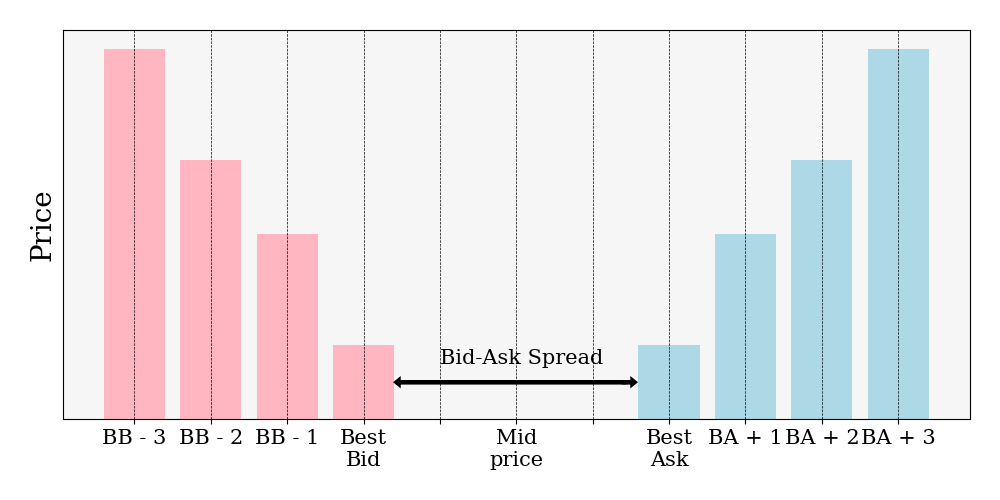
\includegraphics[width=0.8\textwidth]{figures/spread_def.png}
    \end{figure}
\end{frame}

\begin{frame}{Feature 1 : Bid-Ask Spread}
    \begin{itemize}
        \item For each stock and corresponding observations, we plot the mean spread over the 100 events.
    \end{itemize}

    \begin{figure}[H]
        \centering
        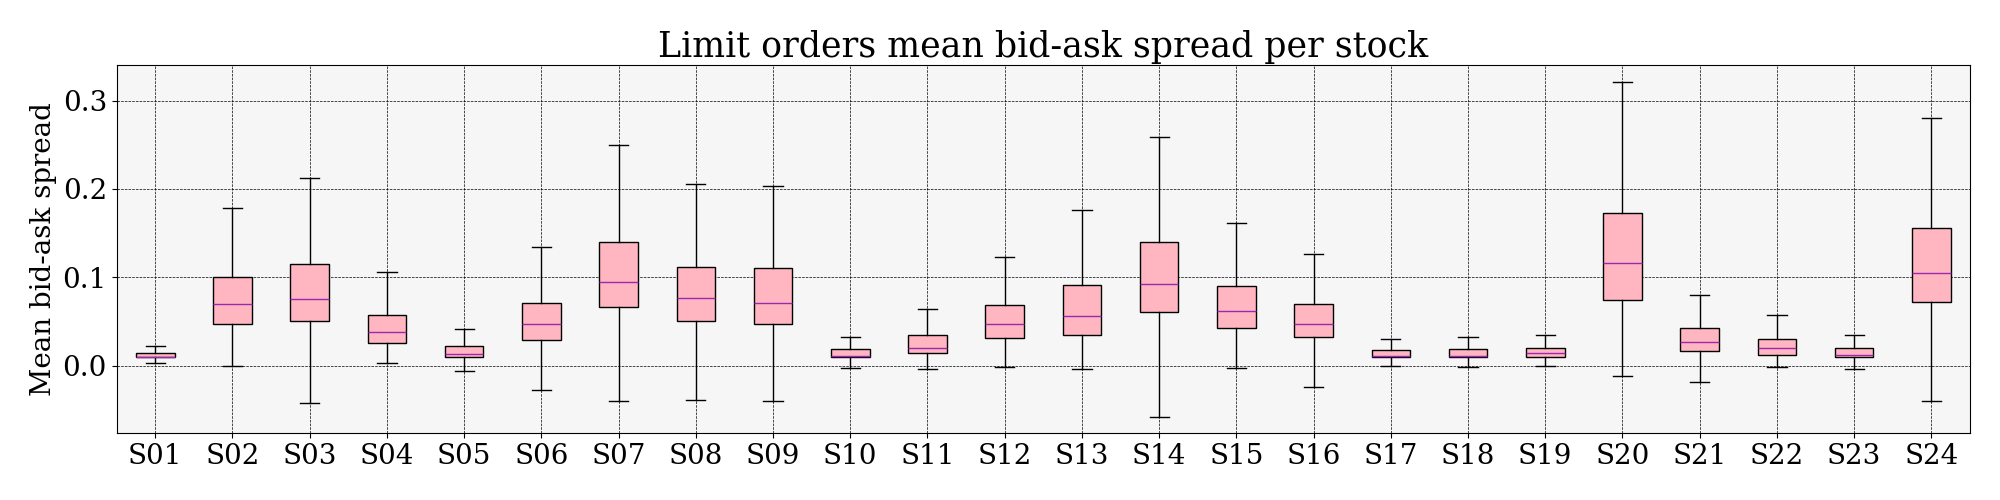
\includegraphics[width=\textwidth]{figures/mean_spread_per_stock_mo.png}
    \end{figure}

    \begin{itemize}
        \myitem The spread is a \textbf{good indicator} of the stock, with a decent variety of boxplot shapes.
        \myitem Most stocks are \textbf{fairly liquid}, with an average spread of less than $10$ ticks.
        \myitem Some stocks are strikingly \textbf{more volatile} than others.
    \end{itemize}
\end{frame}

\begin{frame}{Feature 2 : Best Bid and Ask volumes}
    \begin{itemize}
        \item \textbf{Best Bid and Ask volumes:} Another natural measure of \textbf{liquidity}.
    \end{itemize}
    \begin{figure}[H]
        \centering
        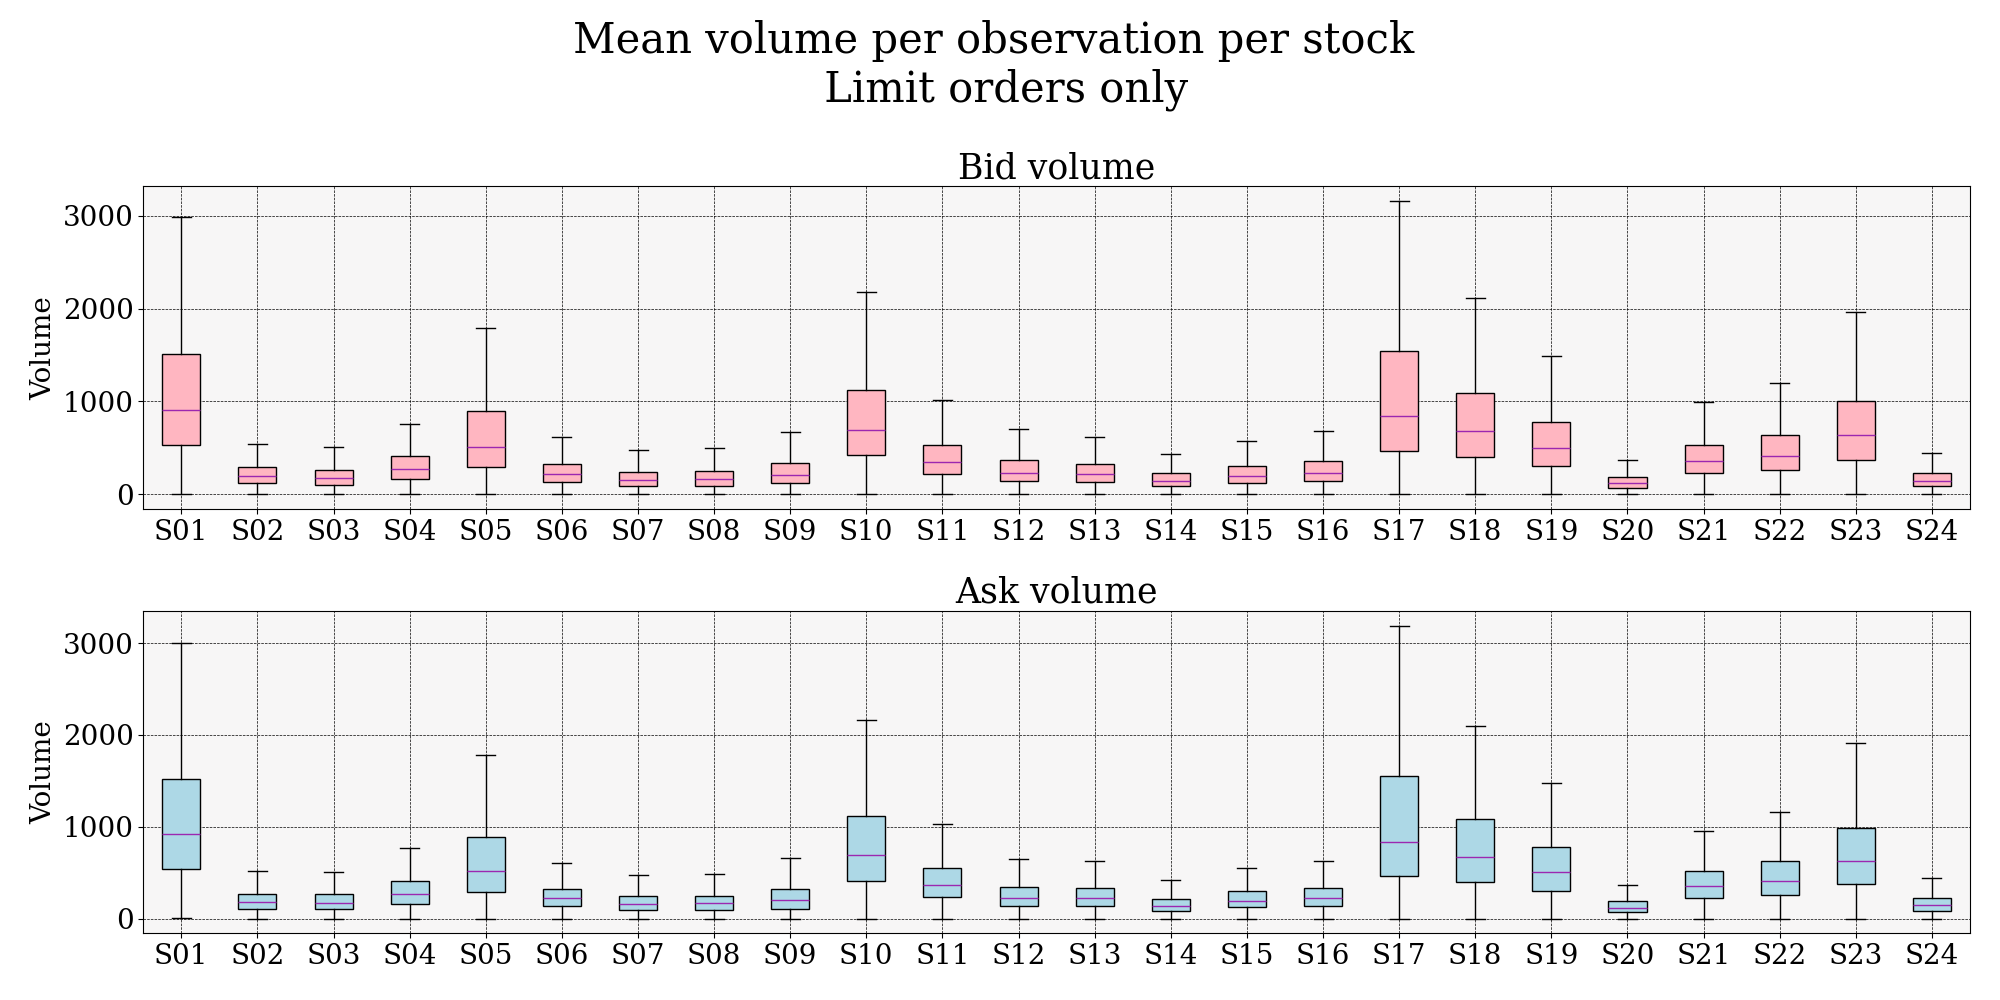
\includegraphics[width=\textwidth]{figures/boxplot_volume_per_stock.png}
    \end{figure}
\end{frame}

\begin{frame}{Feature 3 : Price outliers (number and price value)}
    \begin{itemize}
        \item \textbf{Definition:} A price outlier of order $i$ is a price that is more than $i$ ticks away from the best bid or ask.
              \begin{figure}[H]
                  \centering
                  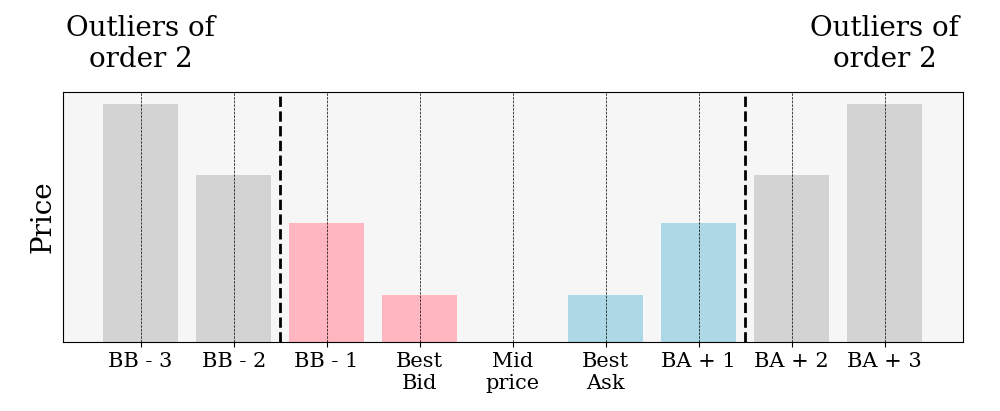
\includegraphics[width=0.6\textwidth]{figures/price_outliers_def.png}
              \end{figure}
              \begin{figure}[H]
                  \centering
                  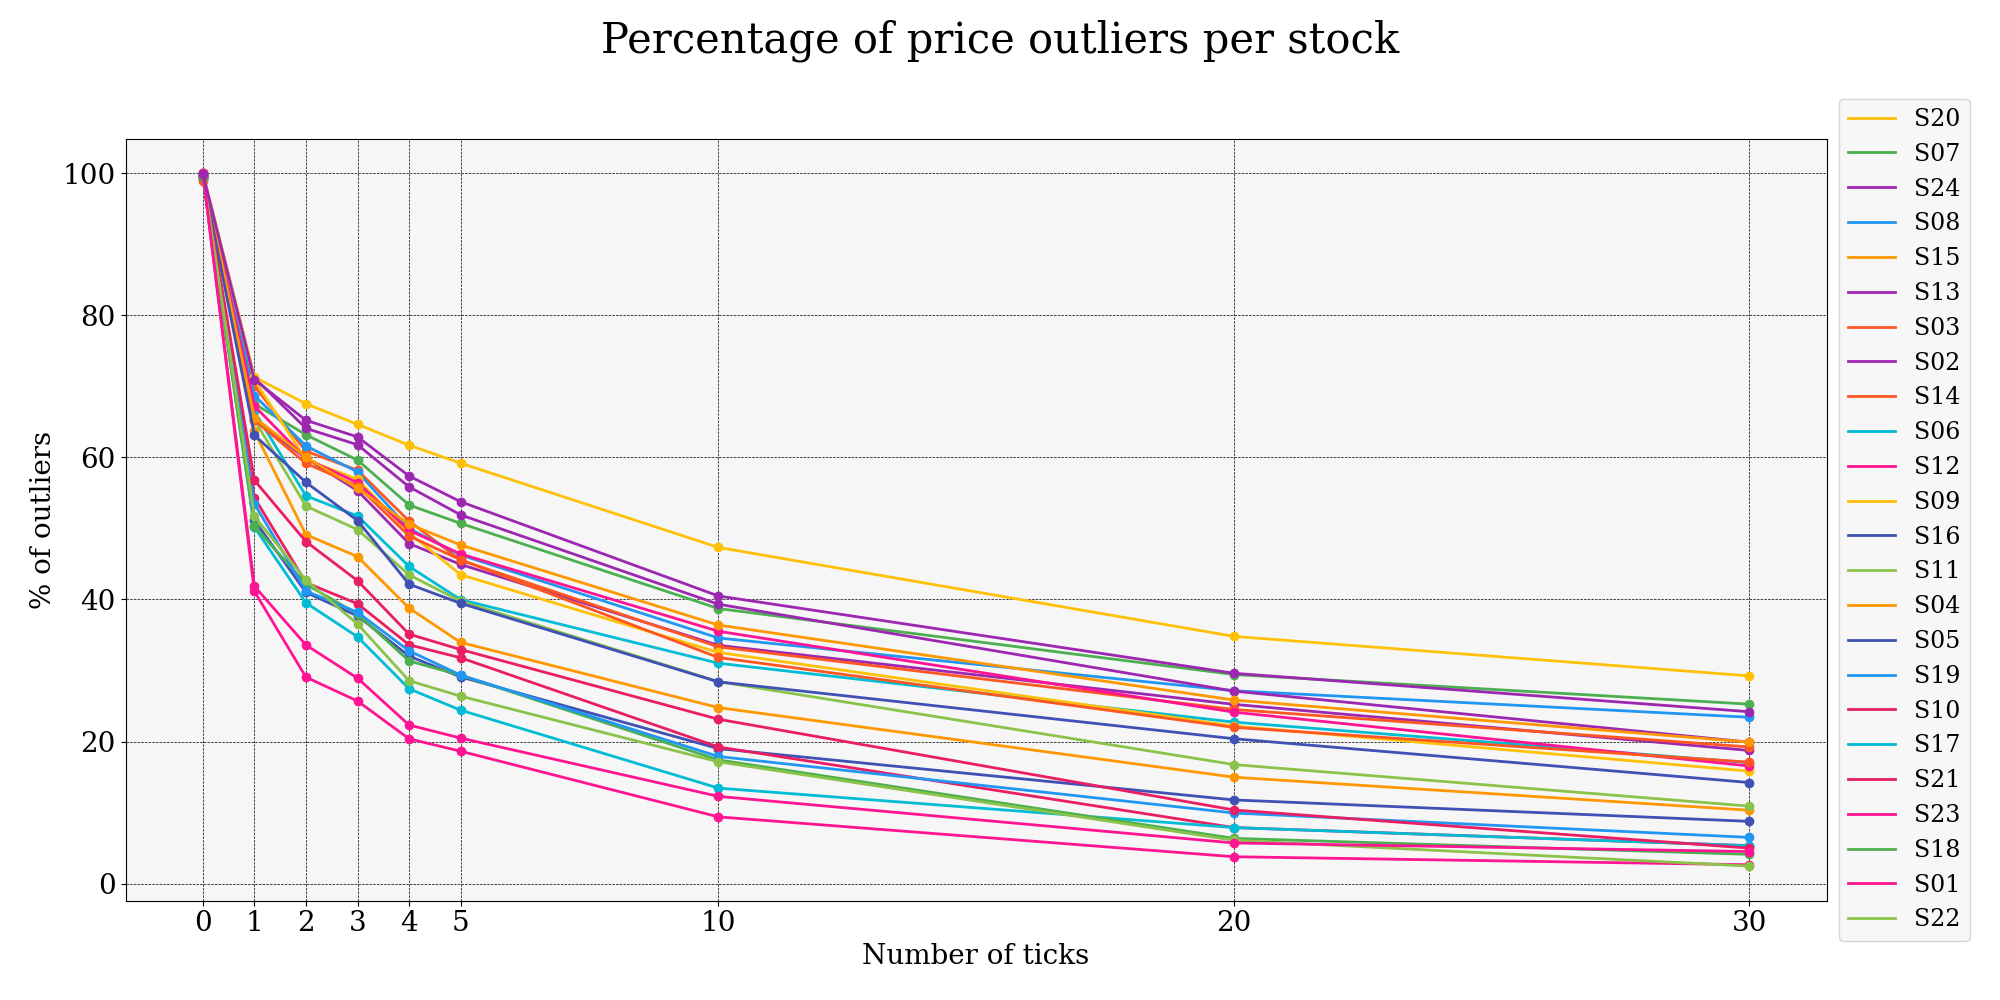
\includegraphics[width=0.7\textwidth]{figures/percentage_outliers_per_stock.png}
              \end{figure}
    \end{itemize}
\end{frame}

\begin{frame}{Feature 3 : Price outliers (number and price value)}
    We plot for each stock and corresponding observations, the mean price value of the outliers over the 100 events.
    \begin{figure}[H]
        \centering
        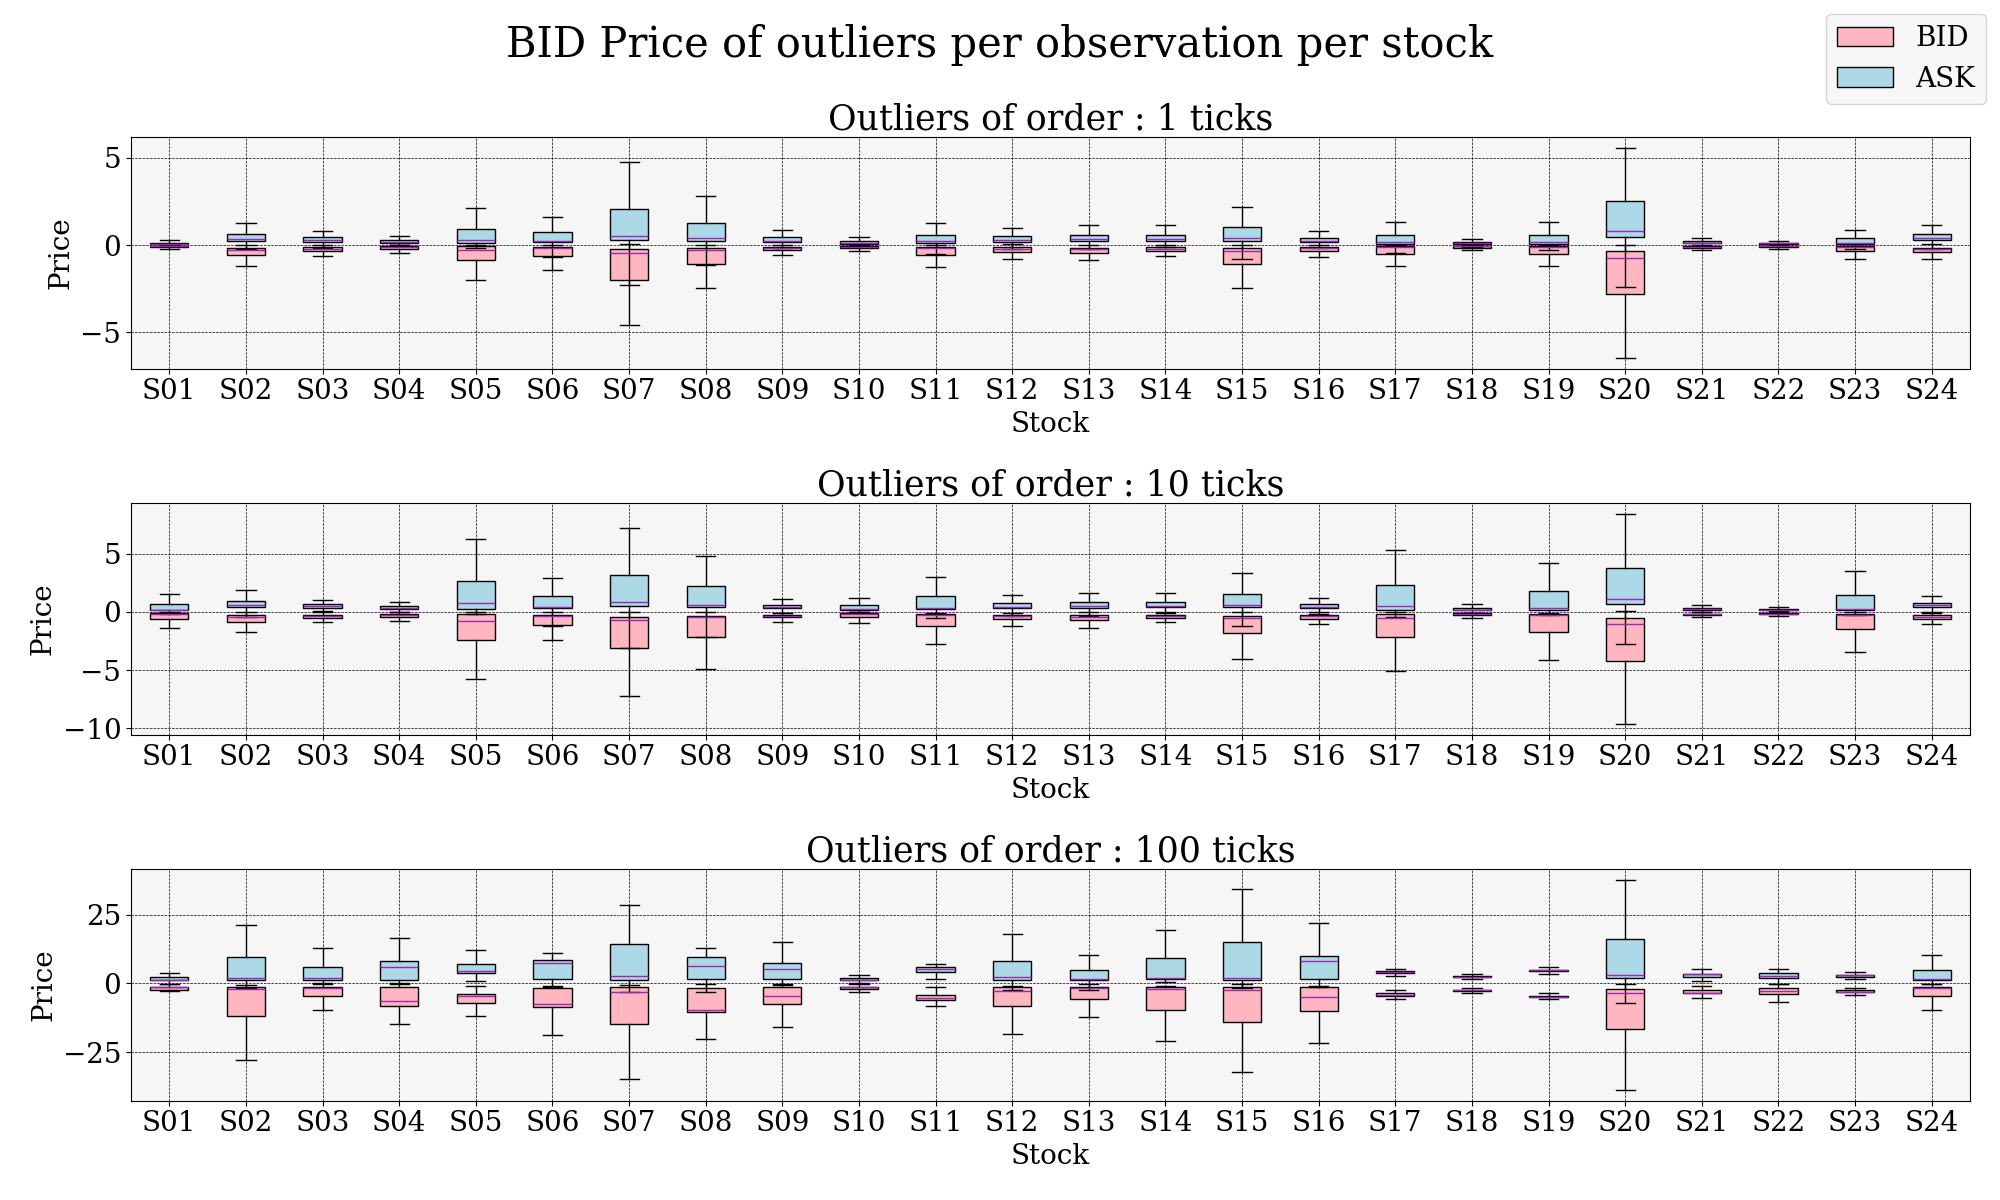
\includegraphics[width=0.87\textwidth]{figures/boxplot_price_outliers_BID_ASK.png}
    \end{figure}
    Some stocks stand out well.
\end{frame}

\begin{frame}{Feature 4 : Price outliers (flow)}
    \begin{itemize}
        \item We plot for each stock and corresponding observations, the mean flow value of the outliers over the 100 events.
        \item Analysis on $4$ subsets of the data: ask addition, ask update, bid update and bid addition.
    \end{itemize}
    \begin{figure}[H]
        \centering
        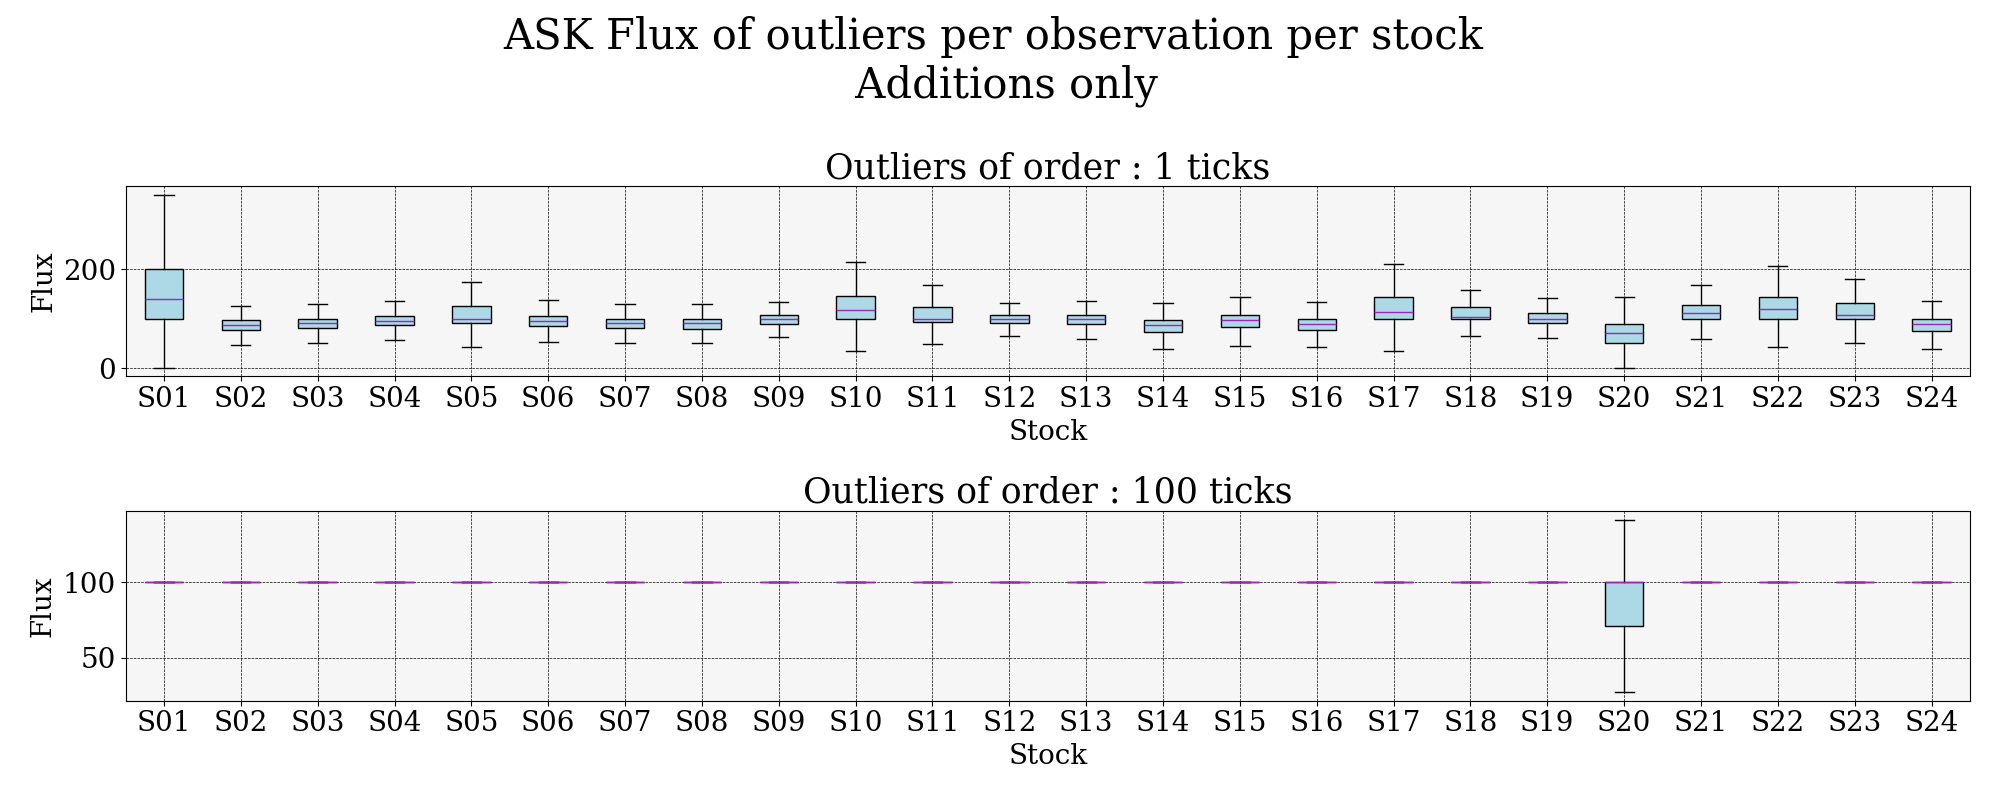
\includegraphics[width=0.9\textwidth]{figures/boxplot_flux_outliers_ASK.png}
    \end{figure}
\end{frame}
\section{Random Forest Classifier and Feature Importance Analysis}
\begin{frame}{Random Forest Classifier}
    A first approach to the classification task is to use a \textbf{Random Forest Classifier} using the hand-crafted features.
    \newline\newline
    \textbf{$2$ objectives:}
    \begin{itemize}
        \item \textbf{Feature importance:} Use the feature importance to unravel the most discriminative features.
        \item \textbf{Performance:} We tested $2$ different models on different sets of features:
              \begin{enumerate}
                  \item \textbf{Model 1's features:} the Bid-Ask spread, the Bid and Ask volume, the number of price outliers, the price outliers, the flux of the price outliers, and the proportion of each venues on which the orders were placed.
                  \item \textbf{Model 2's features:} Only a subset of the features of Model 1: the Bid-Ask spread, the Bid and Ask volume and the venue proportions.
              \end{enumerate}
    \end{itemize}
\end{frame}
\begin{frame}{Feature importance}
    \begin{figure}[H]
        \centering
        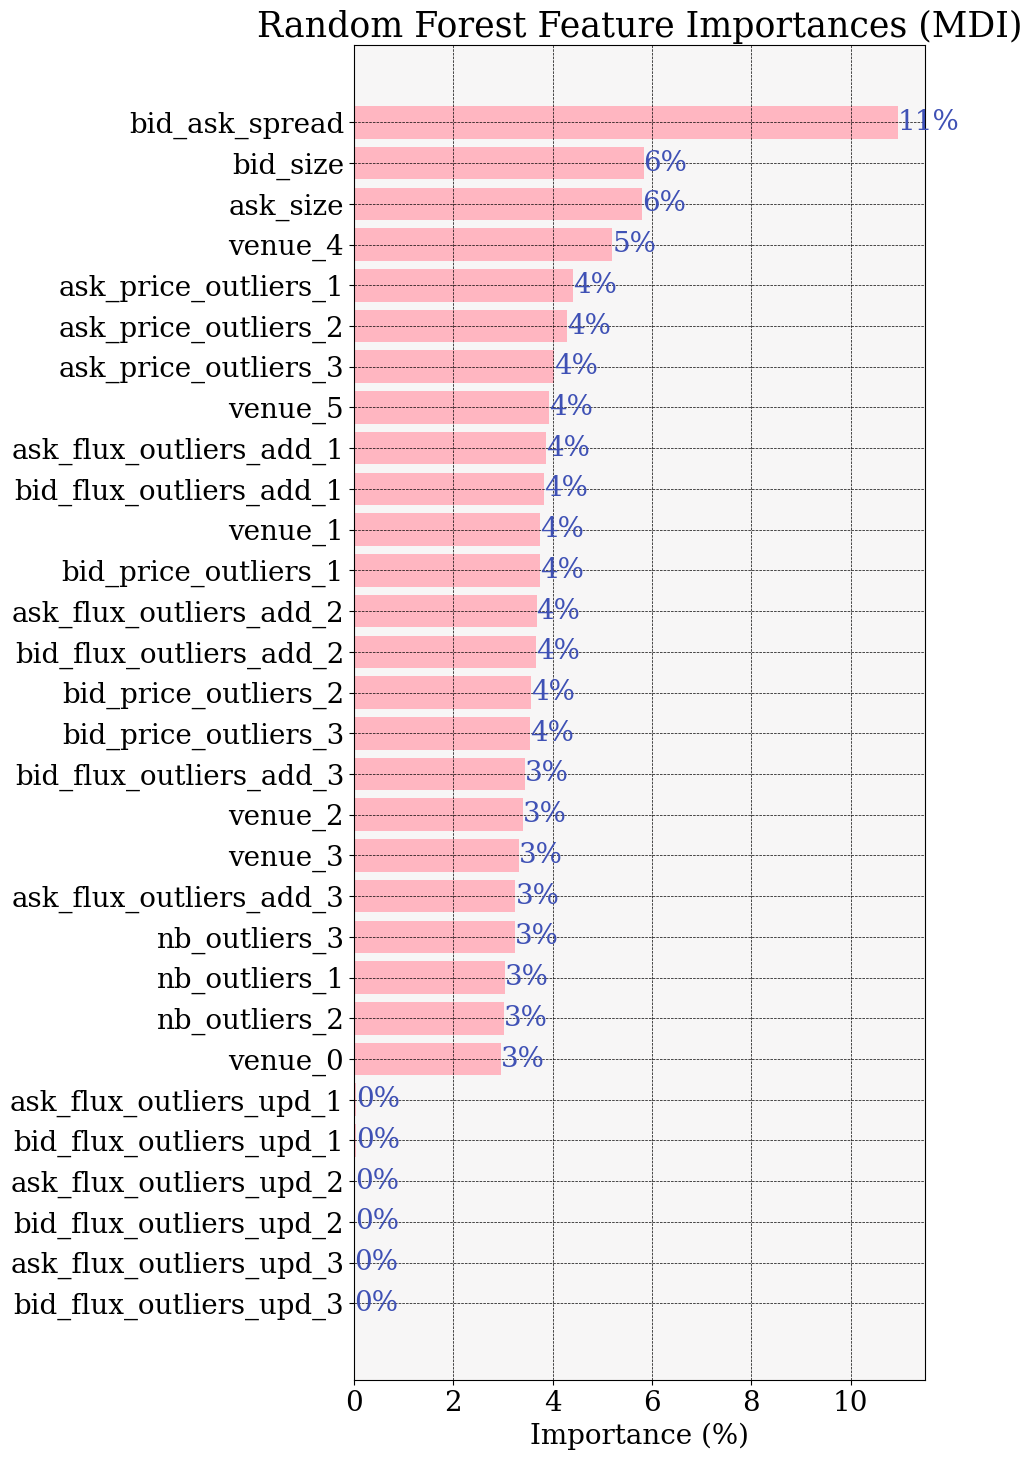
\includegraphics[width=0.5\textwidth]{figures/feature_importance.png}
    \end{figure}
\end{frame}

\begin{frame}{Performance of the $2$ random forest models}
    \begin{table}[H]
        \begin{center}
            \begin{tabular}{|c|c|c|}
                \hline
                \textbf{Model} & \textbf{Validation accuracy} & \textbf{Test accuracy} \\
                \hline
                Model 1        & $49 \%$                      & $22 \%$                \\
                \hline
                Model 2        & $28 \%$                      & $20 \%$                \\
                \hline
            \end{tabular}
        \end{center}
    \end{table}
    $\rightarrow$ \textbf{Conclusion:} Clear indication that the "outlier" features, while being very discriminative on the training set, are almost irrelevant on the test set.
\end{frame}
\section{Feature-based approach}
\begin{frame}{Franck Zibi's model}
    \textbf{Model :} Inspired by the winning solution of last year’s challenge.
    \begin{enumerate}
        \item A random forest classifier is trained on the training set. Outputs a probability distribution over the classes.
        \item Predict the residuals of the random forest classifier for each class using three models (Ridge regressor, k-nearest neighbors regressor, linear regressor).
        \item Stack the three models using a linear regressor.
        \item Predict the class of a sample by adding the output of the random forest classifier to the output of the stacked models, and taking the class with the highest probability.
    \end{enumerate}
\end{frame}

\begin{frame}{Used features}
    Used features for the classification task:
    \begin{enumerate}
        \item Compute min, max, mean, median, and standard deviation over the 100 events : for each of the $11$ original features, as well as the bid-ask spread, the limit order indicator, and the sum of bid and ask sizes.
        \item Add the features we previously engineered:
              \begin{itemize}
                  \item The Bid-ask spread
                  \item The volume of the orders (bid and ask size)
                  \item The number of price outliers
                  \item The average price of the outliers
                  \item The average flux of the price outliers for the different types of outliers (ask addition, ask update, bid update)
                  \item The venue proportions
              \end{itemize}
    \end{enumerate}
\end{frame}

\begin{frame}{Data normalization}
    \begin{enumerate}
        \item Approach based on features engineered with market intuition \checkmark
        \item More generic approach :
    \end{enumerate}
    \vspace{5mm}
    \begin{itemize}
        \item \textbf{Outliers removal} : Remove observations with at least one value at more than $7$ standard deviations from the mean. Removed around $3.6\%$ of the training set.
        \item \textbf{Log transformation} : Applied to the flux, bid size and ask size. Preserves the sign of the values.
        \item \textbf{Min-max scaling} : Further normalization of the bid size and ask size features.
    \end{itemize}
\end{frame}

\section{Graph modelisation approach}
\begin{frame}{Graph representation}
    \begin{itemize}
        \item \textbf{Main idea:} Represent the data as a graph to capture the temporal dependencies between the events, as well as to give a structural representation of the data.
    \end{itemize}
    \begin{figure}[H]
        \centering
        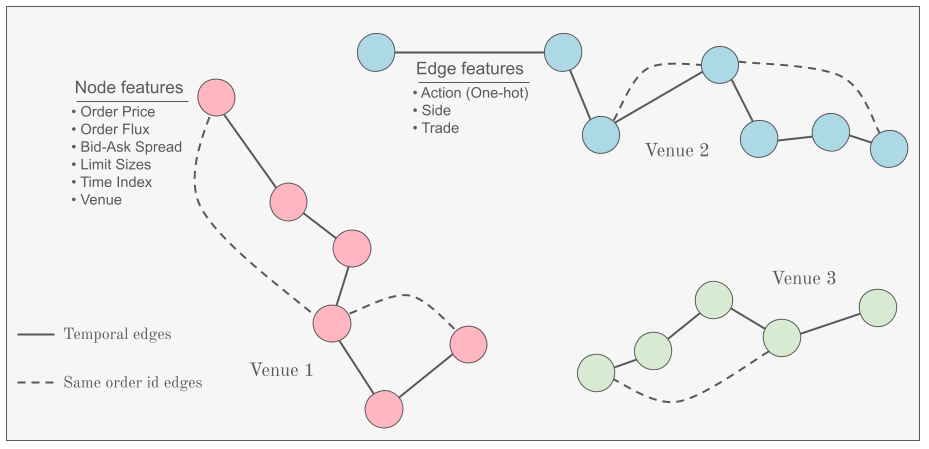
\includegraphics[width=0.8\textwidth]{figures/graph_structure.png}
    \end{figure}
\end{frame}

\begin{frame}{Graph Attention Network (GAT)}
    $G$ : undirected graph with $N$ nodes, node features $h_1, \ldots, h_N \in \mathbb{R}^{d_1}$, edge features $\left\{e_{i,j} \; | 1\leq i,j\leq N\right\} \in\R^{d_2}$
    \begin{block}{Attention weights}
        \begin{equation*}
            w(h_i,h_j, e_{i,j}) = a^T \leakyrelu(W_1h_i + W_1h_j + W_2e_{i,j})
        \end{equation*}
        \begin{equation*}
            \alpha_{ij} = \frac{\exp(w(h_i,h_j, e_{i,j}))}{\sum_{k\in\mathcal{N}_i}\exp(w(h_i,h_k, e_{i,k}))}
        \end{equation*}
        with $\mathcal{N}_i$ the set of neighbors of node $i$, and $W_1$, $W_2$ and $a$ learnable parameters.
    \end{block}
    \begin{block}{Embedding update}
        \begin{equation*}
            h_i' = \leakyrelu\left(\frac{1}{K}\sum_{k=1}^K\sum_{j\in\mathcal{N}_i}\alpha_{ij}^{(k)}W_1^{(k)}h_j\right)
        \end{equation*}
        where $K$ is the number of attention heads.
    \end{block}
\end{frame}

\section{Recurrent Neural Networks approach}
\begin{frame}{LSTM (Long-Short Term Memory)}
    \begin{itemize}
        \item Categorical features embedding
        \item MLP on the last hidden state
        \item Bidirectional
    \end{itemize}
    \begin{figure}
        \centering
        \resizebox{0.6\columnwidth}{!}{
            \begin{tikzpicture}[
                    % GLOBAL CFG
                    font=\sf \scriptsize,
                    >=LaTeX,
                    % Styles
                    cell/.style={% For the main box
                            rectangle,
                            rounded corners=5mm,
                            draw,
                            very thick,
                        },
                    operator/.style={%For operators like +  and  x
                            circle,
                            draw,
                            inner sep=-0.5pt,
                            minimum height =.2cm,
                        },
                    function/.style={%For functions
                            ellipse,
                            draw,
                            inner sep=1pt
                        },
                    ct/.style={% For external inputs and outputs
                            circle,
                            draw,
                            line width = .75pt,
                            minimum width=1cm,
                            inner sep=1pt,
                        },
                    gt/.style={% For internal inputs
                            rectangle,
                            draw,
                            minimum width=4mm,
                            minimum height=3mm,
                            inner sep=1pt
                        },
                    mylabel/.style={% something new that I have learned
                            font=\scriptsize\sffamily
                        },
                    ArrowC1/.style={% Arrows with rounded corners
                            rounded corners=.25cm,
                            thick,
                        },
                    ArrowC2/.style={% Arrows with big rounded corners
                            rounded corners=.5cm,
                            thick,
                        },
                ]

                %Start drawing the thing...    
                % Draw the cell: 
                \node [cell, minimum height =4cm, minimum width=6cm] at (0,0){} ;

                % Draw inputs named ibox#
                \node [gt] (ibox1) at (-2,-0.75) {$\sigma$};
                \node [gt] (ibox2) at (-1.5,-0.75) {$\sigma$};
                \node [gt, minimum width=1cm] (ibox3) at (-0.5,-0.75) {Tanh};
                \node [gt] (ibox4) at (0.5,-0.75) {$\sigma$};

                % Draw opérators   named mux# , add# and func#
                \node [operator] (mux1) at (-2,1.5) {$\times$};
                \node [operator] (add1) at (-0.5,1.5) {+};
                \node [operator] (mux2) at (-0.5,0) {$\times$};
                \node [operator] (mux3) at (1.5,0) {$\times$};
                \node [function] (func1) at (1.5,0.75) {Tanh};

                % Draw External inputs? named as basis c,h,x
                \node[ct, label={[mylabel]Cell}] (c) at (-4,1.5) {\empt{c}{t-1}};
                \node[ct, label={[mylabel]Hidden}] (h) at (-4,-1.5) {\empt{h}{t-1}};
                \node[ct, label={[mylabel]left:Input}] (x) at (-2.5,-3) {\empt{x}{t}};

                % Draw External outputs? named as basis c2,h2,x2
                \node[ct] (c2) at (4,1.5) {\empt{c}{t}};
                \node[ct] (h2) at (4,-1.5) {\empt{h}{t}};
                \node[ct] (x2) at (2.5,3) {\empt{h}{t}};

                % Start connecting all.
                %Intersections and displacements are used. 
                % Drawing arrows    
                \draw [ArrowC1] (c) -- (mux1) -- (add1) -- (c2);

                % Inputs
                \draw [ArrowC2] (h) -| (ibox4);
                \draw [ArrowC1] (h -| ibox1)++(-0.5,0) -| (ibox1);
                \draw [ArrowC1] (h -| ibox2)++(-0.5,0) -| (ibox2);
                \draw [ArrowC1] (h -| ibox3)++(-0.5,0) -| (ibox3);
                \draw [ArrowC1] (x) -- (x |- h)-| (ibox3);

                % Internal
                \draw [->, ArrowC2] (ibox1) -- (mux1);
                \draw [->, ArrowC2] (ibox2) |- (mux2);
                \draw [->, ArrowC2] (ibox3) -- (mux2);
                \draw [->, ArrowC2] (ibox4) |- (mux3);
                \draw [->, ArrowC2] (mux2) -- (add1);
                \draw [->, ArrowC1] (add1 -| func1)++(-0.5,0) -| (func1);
                \draw [->, ArrowC2] (func1) -- (mux3);

                %Outputs
                \draw [-, ArrowC2] (mux3) |- (h2);
                \draw (c2 -| x2) ++(0,-0.1) coordinate (i1);
                \draw [-, ArrowC2] (h2 -| x2)++(-0.5,0) -| (i1);
                \draw [-, ArrowC2] (i1)++(0,0.2) -- (x2);

            \end{tikzpicture}
        }
        \caption{LSTM cell diagram}
    \end{figure}
\end{frame}

\section{Training of Graph models and RNNs}

\begin{frame}{Loss}
    \begin{itemize}
        \item Cross-entropy loss
        \item Minimum class confusion (MCC) loss on the test set
    \end{itemize}

    \begin{block}{MCC}
        Batch of samples $(X_n)_{1\leq n\leq N}$ and model predictions $\hat{Y}_n = F(X_n)\in\R^{24}$ :

        \begin{minipage}{.5\linewidth}
            \begin{equation*}
                \textbf{1.}\:\: \tilde{Y}_{n,i} = \frac{\exp\left(\hat{Y}_{n,i}/T\right)}{\sum_{j=1}^{24}\exp\left(\hat{Y}_{n,j}/T\right)}
            \end{equation*}
            \vspace*{\fill}
        \end{minipage}
        \begin{minipage}{.5\linewidth}
            \begin{equation*}
                \textbf{2.}\:\: H_n = -\sum_{i=1}^{24}\tilde{Y}_{n,i}\log\left(\tilde{Y}_{n,i}\right)
            \end{equation*}
            \vspace*{\fill}
        \end{minipage}
        \begin{minipage}{.5\linewidth}
            \begin{equation*}
                \textbf{3.}\:\: W_n = N\times\frac{1+\exp(-H_n)}{\sum_{i=1}^{N} 1+\exp(-H_i)}
            \end{equation*}
            \vspace*{\fill}
        \end{minipage}
        \begin{minipage}{.5\linewidth}
            \begin{equation*}
                \textbf{4.}\:\: C_{i,j} = \tilde{Y}_{\cdot,i}^T \text{diag}(W_1,\dots,W_B) \tilde{Y}_{\cdot,j}
            \end{equation*}
            \vspace*{\fill}
        \end{minipage}
    \end{block}
\end{frame}

\begin{frame}{Model calibration}
    \begin{itemize}
        \item Calibration adjusts model output to match true probabilities.
        \item Calibration performed on validation data to avoid bias.
        \item Isotonic regression chosen for simplicity and effectiveness.
        \item Fits piecewise constant non-decreasing function to data.
    \end{itemize}

    \begin{figure}[H]
        \centering
        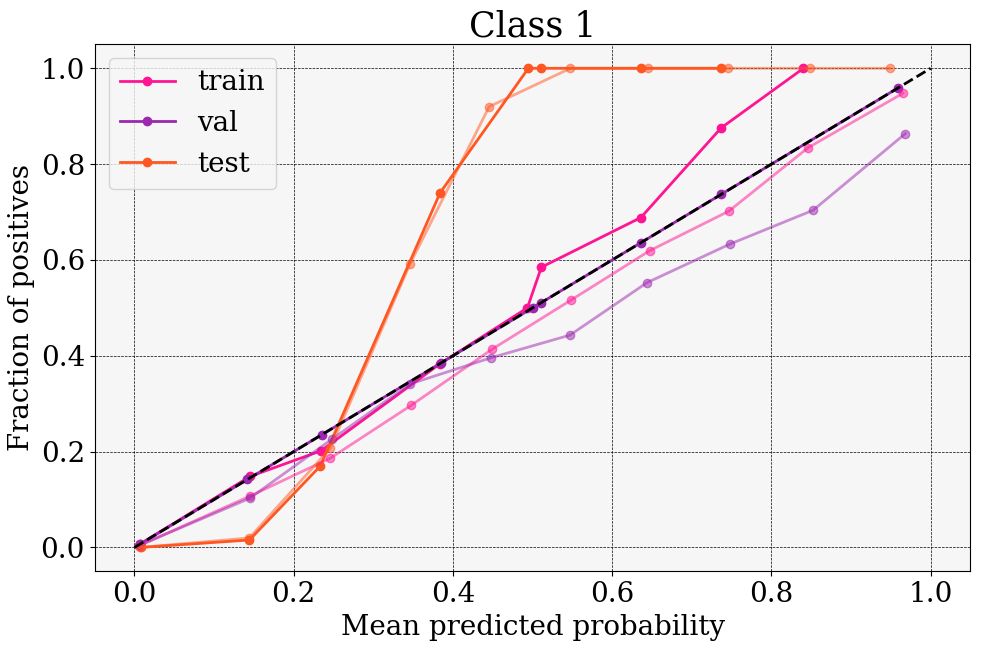
\includegraphics[width=0.6\textwidth]{figures/small_calibration.png}
        \caption{Calibration of the first class of the GAT model.}
        \label{fig:calibration}
    \end{figure}
\end{frame}

\begin{frame}{Training curves}
    \begin{itemize}
        \item Training with Adam, learning rate $5\cdot 10^{-3}$, multiplicative learning rate scheduler ($\times0.95$ per epoch).
        \item Training on RTX4060 with batch size $256$.
    \end{itemize}
    \begin{figure}[H]
        \centering
        \begin{subfigure}{0.49\columnwidth}
            \centering
            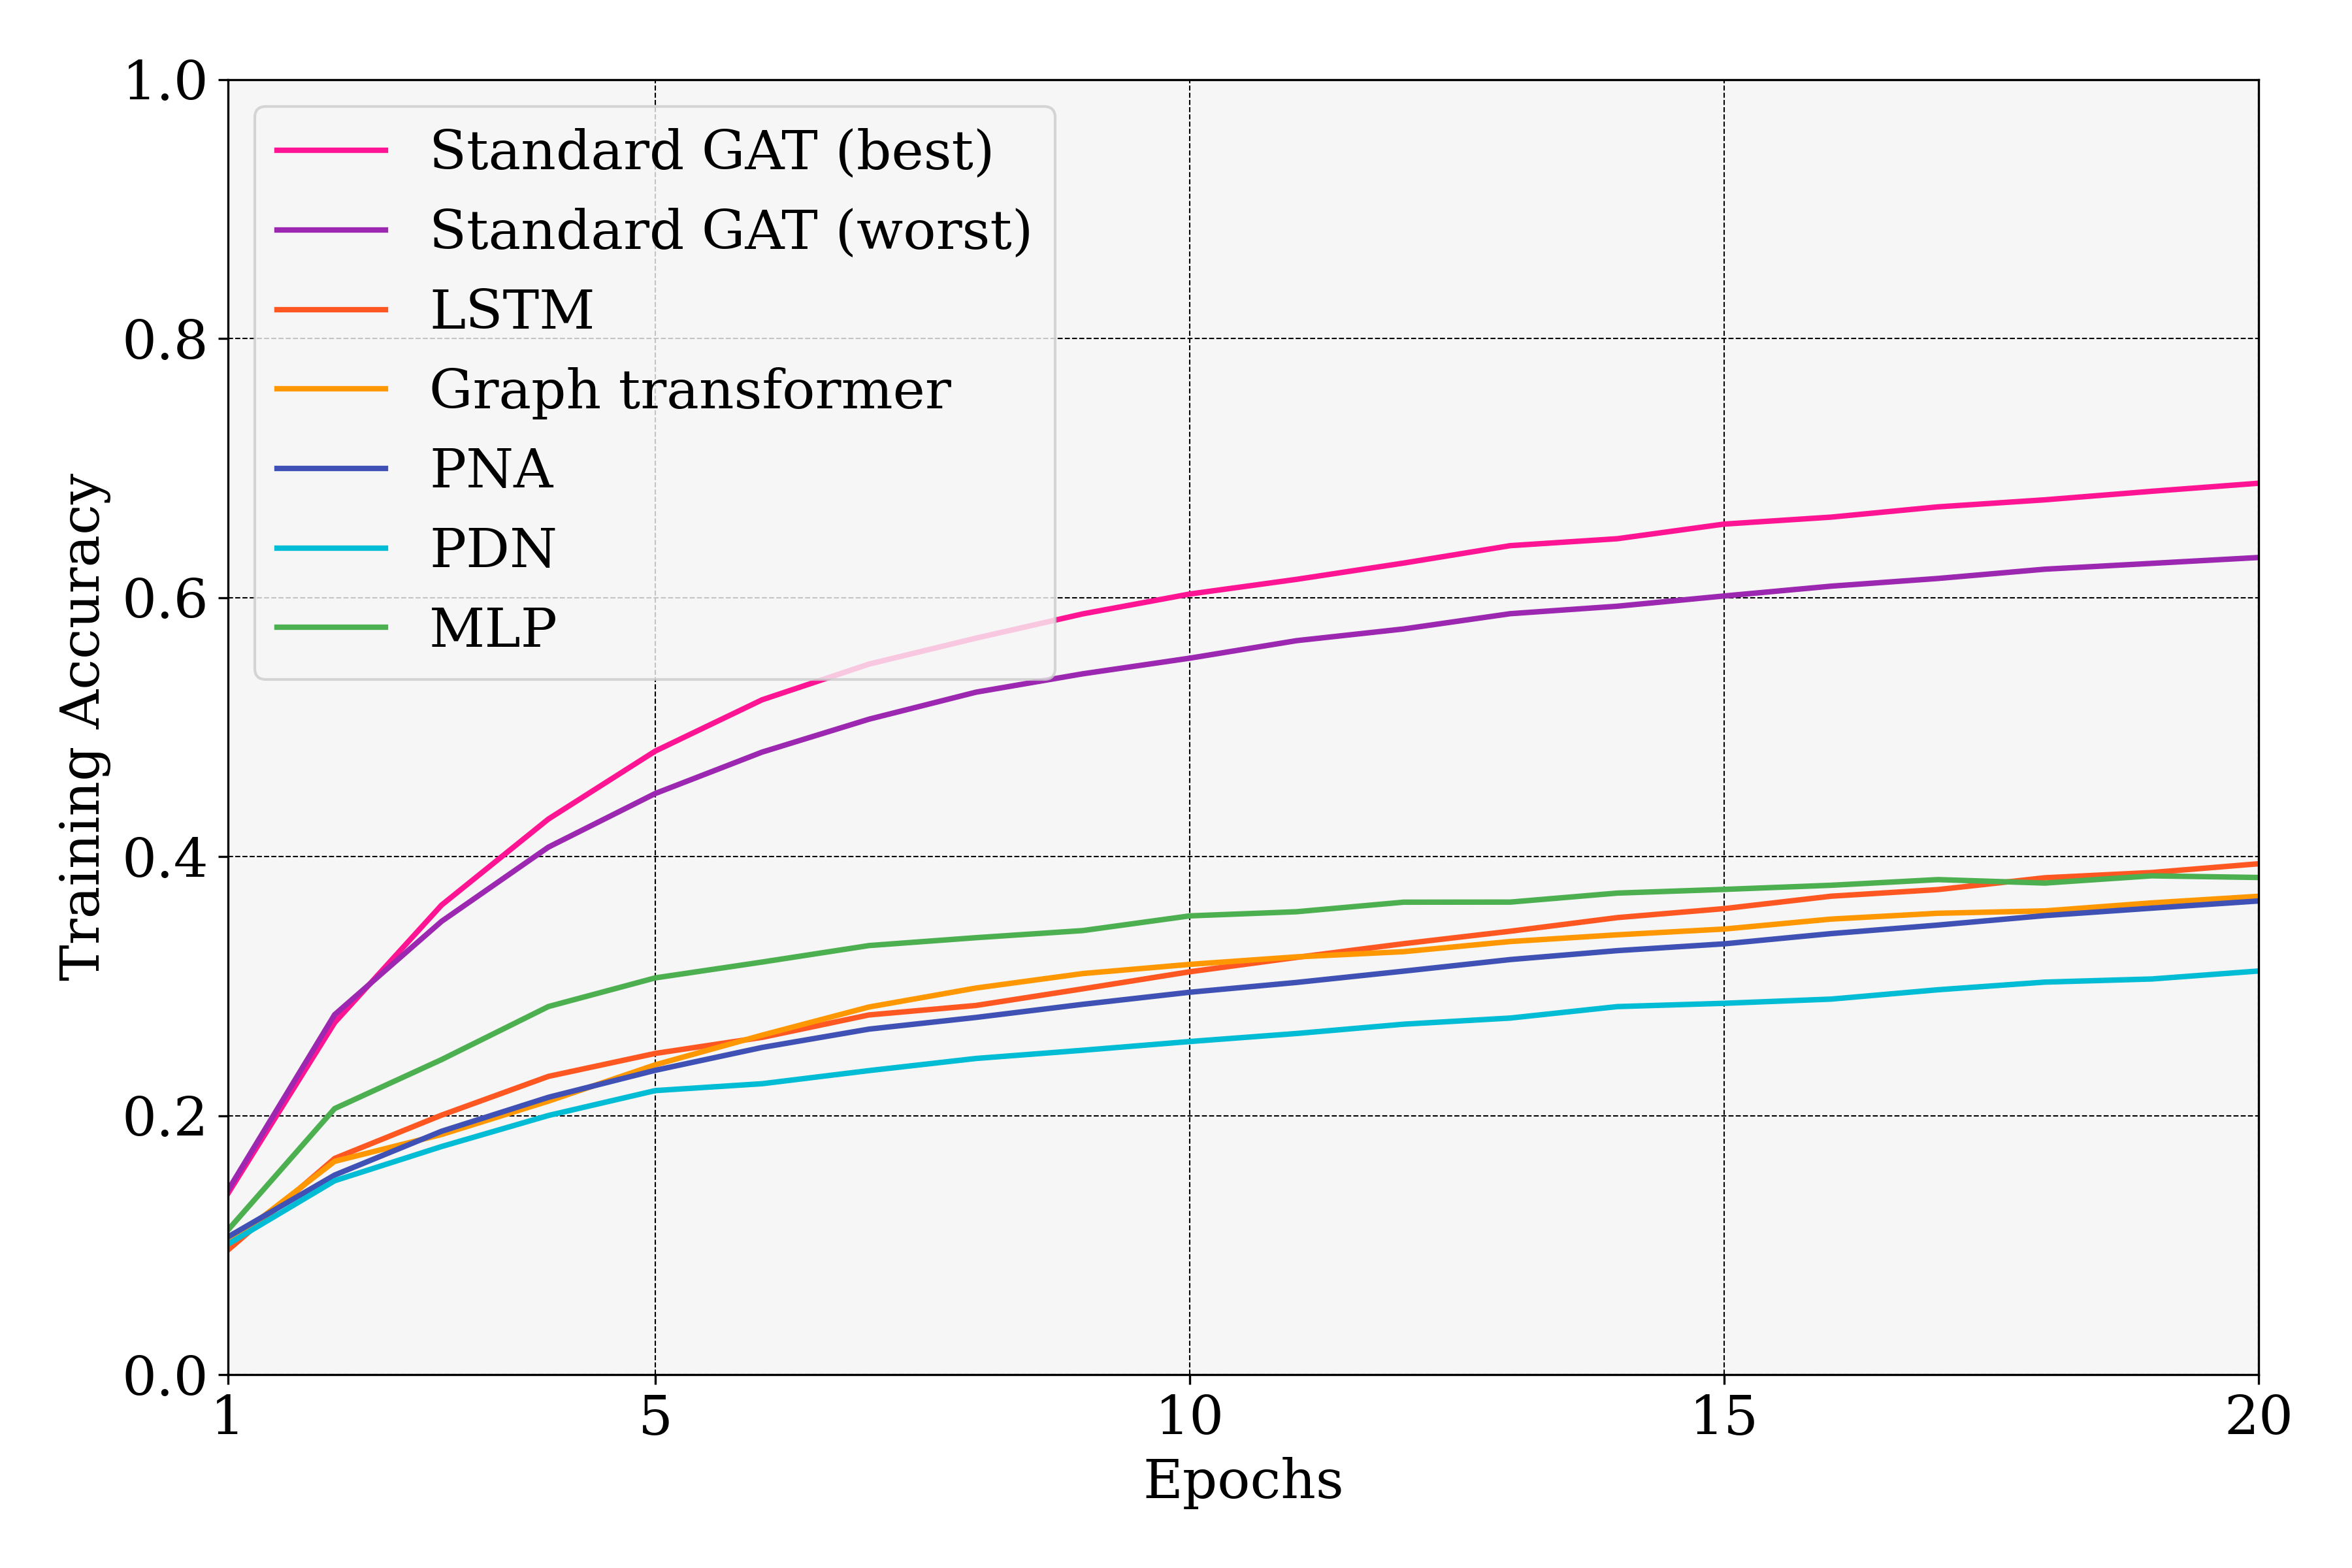
\includegraphics[width=\columnwidth]{figures/train_accuracy.png}
            \caption{Training accuracy}
            \label{fig:train_accuracy}
        \end{subfigure}
        \begin{subfigure}{0.49\columnwidth}
            \centering
            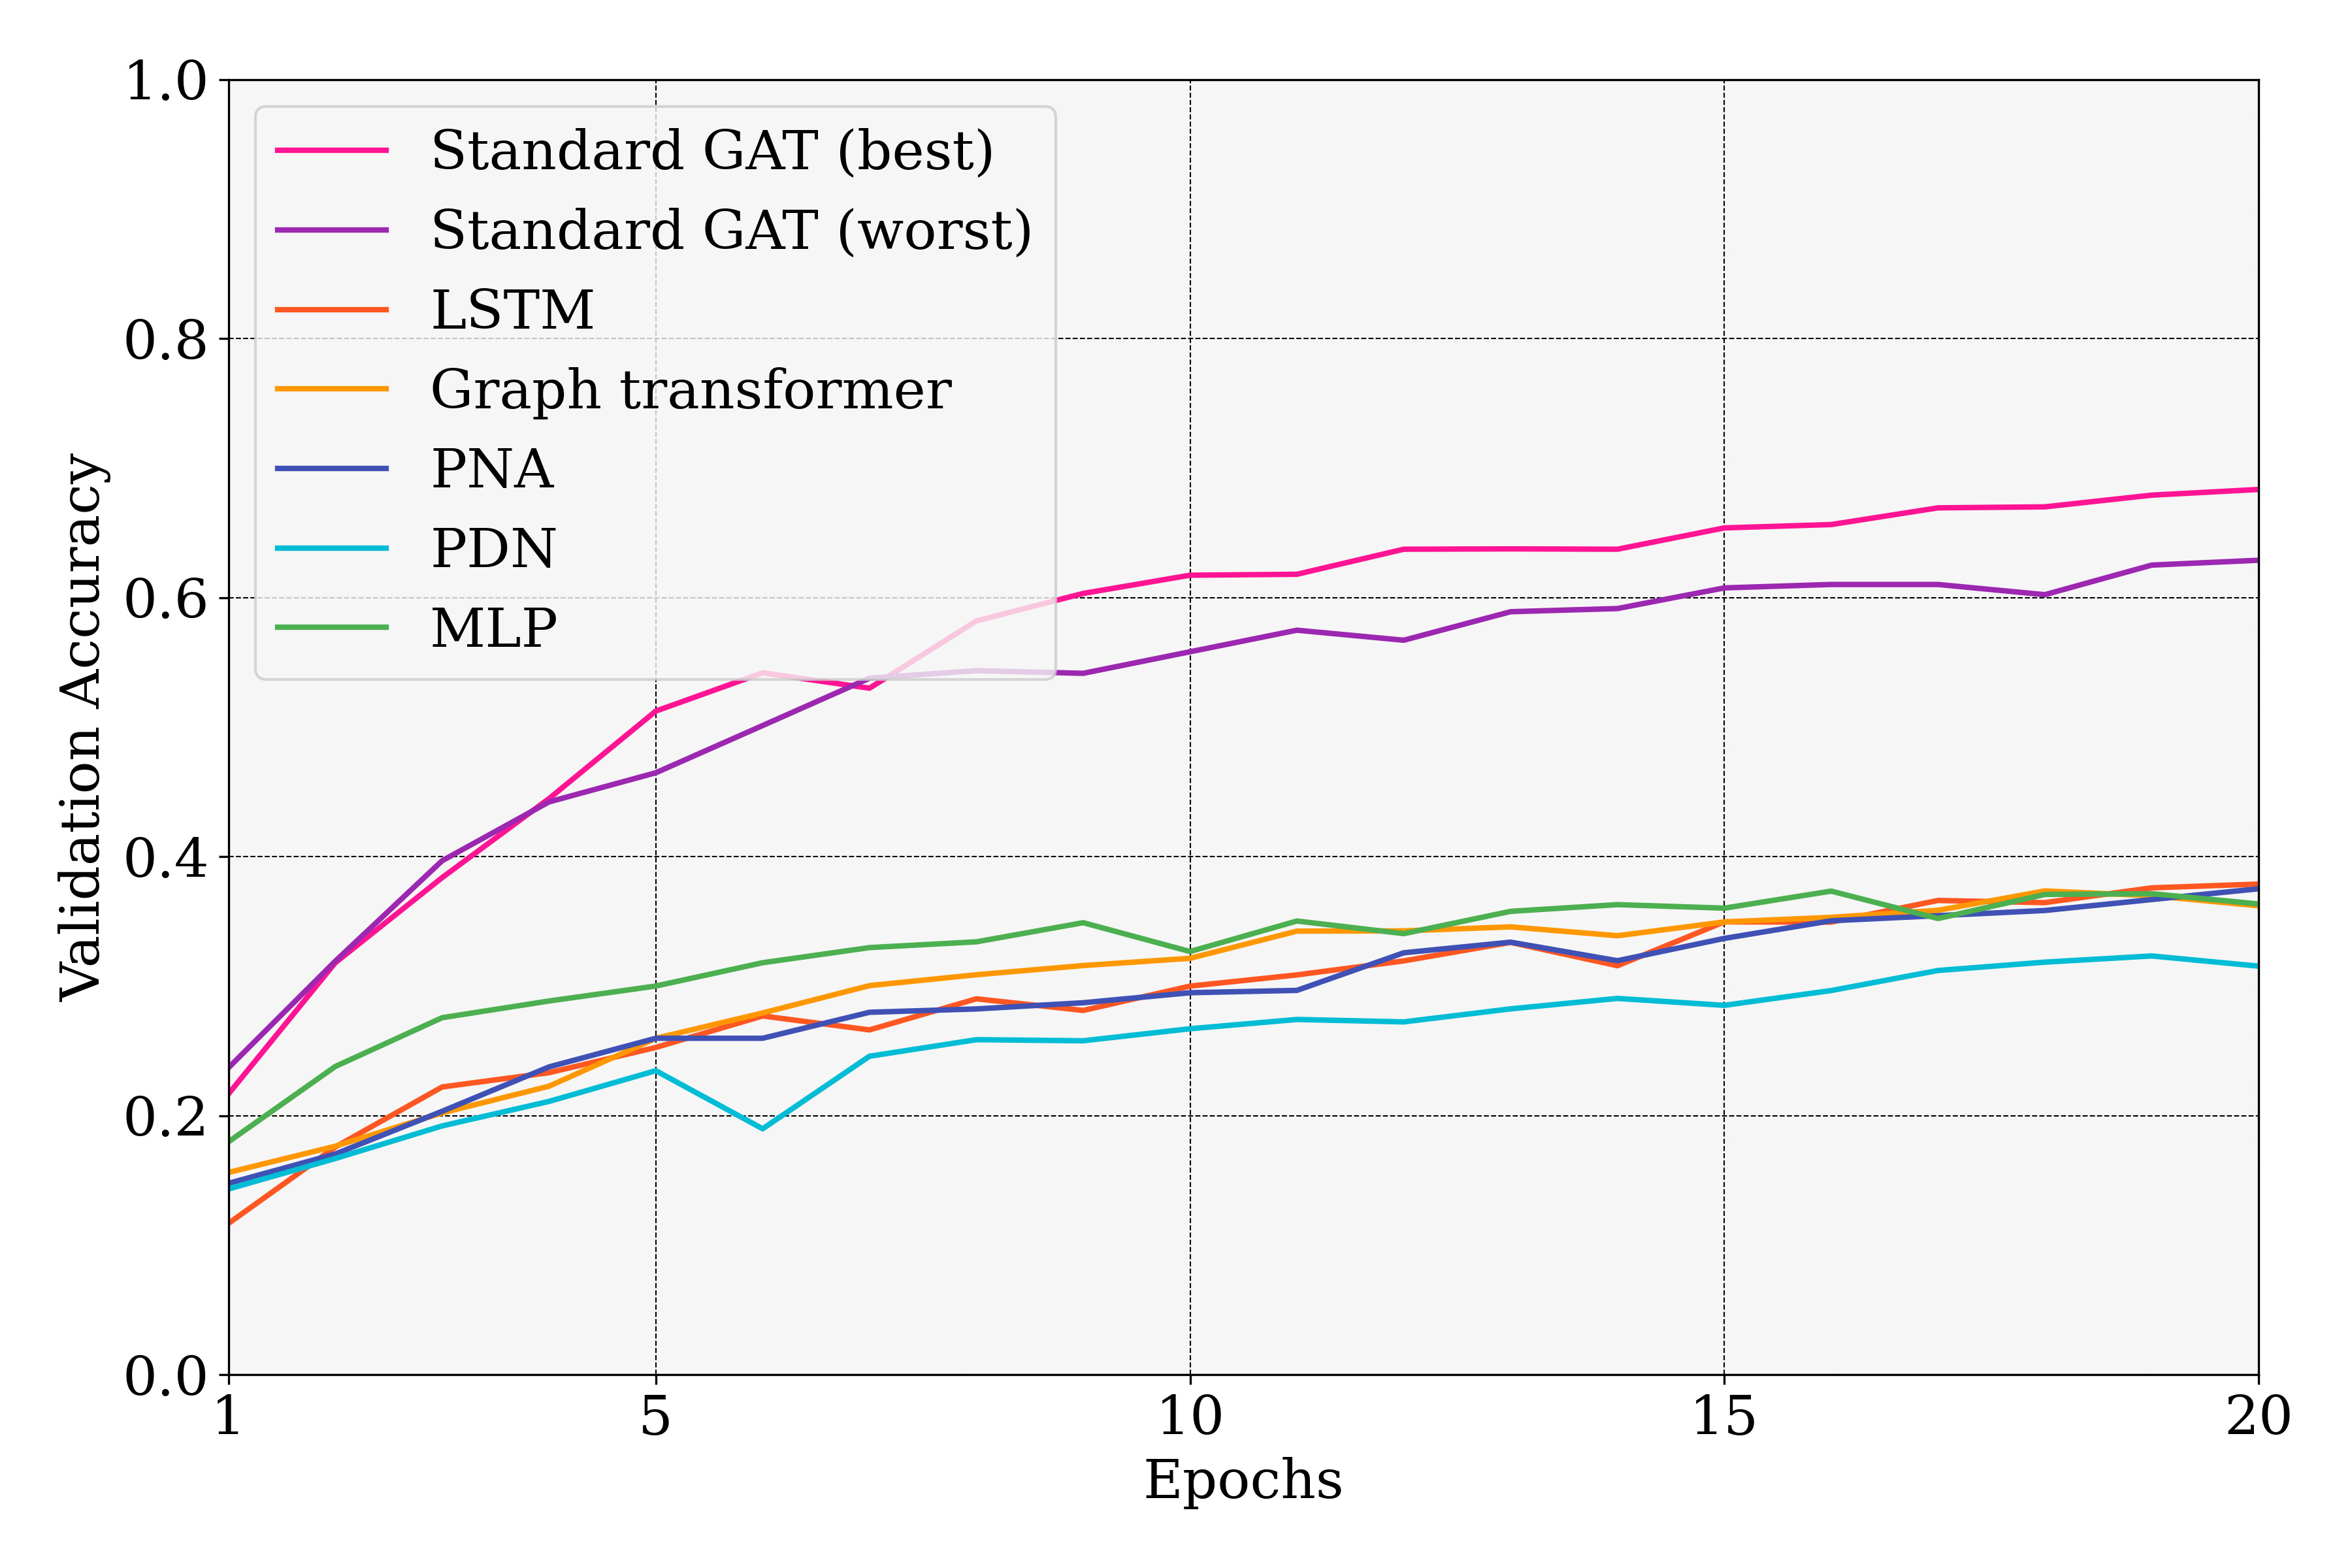
\includegraphics[width=\columnwidth]{figures/val_accuracy.png}
            \caption{Validation accuracy}
            \label{fig:val_accuracy}
        \end{subfigure}
    \end{figure}
\end{frame}

\section{Results}
\begin{frame}{Ensemble Results}
    \begin{table}[H]
        \begin{center}
            \resizebox{\columnwidth}{!}{
                \begin{tabular}{|c|c|c|c|}
                    \hline
                    \textbf{Model description} & \textbf{Training acc.} & \textbf{Validation acc.} & \textbf{Test acc.} \\
                    \hline
                    Random Forest I            & 0.31                   & 0.28                     & 0.19               \\
                    \hline
                    Random Forest II           & 0.50                   & 0.48                     & 0.22               \\
                    \hline
                    PDN                        & 0.42                   & 0.43                     & 0.23               \\
                    \hline
                    MLP                        & 0.42                   & 0.41                     & 0.24               \\
                    \hline
                    Franck Zibi's model        & 0.95                   & 0.42                     & 0.25               \\
                    \hline
                    Graph transformer          & 0.44                   & 0.43                     & 0.29               \\
                    \hline
                    General GNN                & 0.43                   & 0.42                     & 0.30               \\
                    \hline
                    PNA                        & 0.47                   & 0.45                     & 0.30               \\
                    \hline
                    LSTM                       & 0.57                   & 0.44                     & 0.30               \\
                    \hline
                    GAT (50 epochs)            & 0.75                   & 0.71                     & 0.33               \\
                    \hline
                    GAT (20 epochs)            & 0.72                   & 0.68                     & 0.34               \\
                    \hline
                    Generalized GNN            & 0.73                   & 0.71                     & 0.35               \\
                    \hline
                    \textbf{Final ensemble}    & \textbf{0.83}          & \textbf{0.81}            & \textbf{0.40}      \\
                    \hline
                \end{tabular}
            }
        \end{center}
        \caption{Main accuracy results}
        \label{tab:results}
    \end{table}
\end{frame}
\section{Conclusion}
\begin{frame}{Conclusion}
    \textbf{Throughout this challenge, we did:}
    \begin{itemize}
        \item Perform a thorough analysis of the data (visualizations, statistical tests).
        \item Engineer some features that were very discriminative on the training set.
        \item Train a wide variety of models to diversify our ensemble (RNNs, GNNs, statistical models, Franck Zibi's model).
        \item Experiment with different loss functions to make the models more robust to the change of distribution between the training and the test set.
        \item Monitor the training of the models with multiple metrics.
        \item Look into the predictions of the models to try to understand why they were so bad.
    \end{itemize}
\end{frame}

\begin{frame}{Discussion}
    \textbf{Discussion:}
    \begin{itemize}
        \item We achieved over $80\%$ accuracy on the validation set with an ensemble of models.
        \item We achieved a $40\%$ accuracy on the test set.
        \item Main reason for the low accuracy: the change of distribution between the training and the test set.
        \item An interesting approach would be to train a model free of all the "outlier" features, but on a granular level (i.e. by deleting events and not whole samples).
        \item Ninth place on the public leaderboard and a second place on the academic leaderboard.
        \item Some students were able to reach as high as $60\%$ accuracy on the test set. We would be very interested in understanding how they achieved this.
    \end{itemize}
\end{frame}



\end{document}